% =====================================================================
%  Treść (body) — TYLKO sekcje/akapity. Bez preambuły, bez \begin{document}.
%  To jest plik, który piszesz. Wygląd ogarnia formatka.
% =====================================================================

\begin{abstract}
\noindent Krótkie streszczenie (3--5 zdań): co badamy, na jakich danych,
jaki wynik. Empiria, nie deklaracje --- każda teza z dowodem.
\end{abstract}

\section{Wprowadzenie}
Po co ten dokument i jakie pytanie stawiamy. Jedno zdanie tezy + jak ją
zweryfikujemy (pomiar). Powiązanie z nitką dialektyczną (Teza $\to$ Synteza).

\section{Metoda}
Skąd dane, jak je przetwarzamy, jaki model/eksperyment. Definicje formalnie ---
np. metryka błędu $\mathrm{MAE} = \frac{1}{N}\sum_i |\hat{y}_i - y_i|$.
Znaczki matematyczne zawsze w~LaTeX: $\perp$, $\le$, $\alpha$, $\Delta$, $\sum$ --- nigdy unicode.

\section{Wyniki}
Tu ląduje empiria: wykresy + tabele z \emph{liczbami}.

\begin{table}[h]
  \centering
  \caption{Przykładowa tabela wyników (do podmiany na realne).}
  \label{tab:wyniki}
  \begin{tabular}{lrr}
    \toprule
    Wariant & metryka $\downarrow$ & próbek \\
    \midrule
    baseline   & 1.80 & --- \\
    nasz model & 1.20 & --- \\
    \bottomrule
  \end{tabular}
\end{table}

\begin{figure}[h]
  \centering
  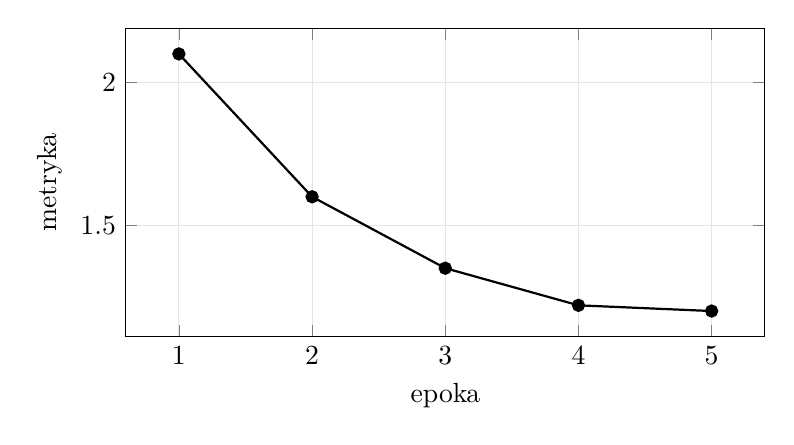
\begin{tikzpicture}
    \begin{axis}[width=0.8\linewidth,height=5.5cm,
        xlabel={epoka}, ylabel={metryka}, grid=both, grid style={gray!20}]
      \addplot[thick,mark=*] coordinates {(1,2.1)(2,1.6)(3,1.35)(4,1.22)(5,1.20)};
    \end{axis}
  \end{tikzpicture}
  \caption{Krzywa uczenia (dane przykładowe).}
  \label{fig:learning}
\end{figure}

Odwołania w tekście: rys.~\ref{fig:hero}, rys.~\ref{fig:learning}, tab.~\ref{tab:wyniki}.

\section{Warunek obalenia}
% Bramka empiryczna metody (patrz README + docs/INSTRUKCJA). NIE usuwaj tej sekcji:
% każda synteza musi nieść test/liczbę/próg, który mógłby ją wywrócić.
Co konkretnie sfalsyfikowałoby tezę: test, liczba albo próg, który mógł wyjść
inaczej. Np. ,,jeśli metryka na held-oucie $>X$, teza upada''. Bez tego synteza
jest co najwyżej zrozumiana ($\to$ bramka epistemiczna), a nie sprawdzona.
Tu wpisz, jak wynik mógł Cię obalić --- i czy Cię nie obalił.

\section{Dyskusja}
Co wynik oznacza, gdzie się nie broni, co dalej. Uczciwie o ograniczeniach
--- spójnie z antytezą nitki.

\section*{Podpis}
Dokument autorstwa: \emph{Autor / kolektyw Slayer}. Skompilowany w~CI.
